\documentclass{article}
\usepackage{graphicx} %package to manage images
\usepackage[utf8]{inputenc}
\usepackage[a4paper, total={6in, 8in}]{geometry}
\usepackage{xurl}
\title{Relatório 8 \\ Análise de qualidade}
\author{Pedro A. S. O. Neto}
\date{Abril, 2022}

\begin{document}

\maketitle

\section{Método}

Fixações perdidas são momentos nos quais o Eye-tracker não detectou o olho do participante. Toda vez que há uma piscada, ou que o participante olha para algum lugar fora da tela, o 
Tobii indica "EyeNotFound". Nesta análise de qualidade, calcula-se o total de fixações perdidas em relação à totalidade do experimento. Foram realizadas duas análises: 

\begin{itemize}
  \item Apenas dos trials de interesse (as trials que serão utilizadas nas análises finais)
  \item Incluindo trials de transição e baseline.
\end{itemize}

Todas as análises foram feitas a nível de indivíduo. Ou seja, os resultados indicam a proporção de EyesFound para EyesNotFound para cada indivíduo, ao longo de todo o experimento.

\begin{table}[!ht]
    \centering
    \caption{Estatísticas descritivas}
    \begin{tabular}{|l|l|l|l|l|}
    \hline
         & media & min & max & sd \\ \hline
        Trials de interesse & 61.01 & 0.74 & 98.54 & 27.38 \\
        Incluindo baseline & 58.78 & 1.72 & 98.36 & 28.13 \\ \hline
    \end{tabular}
\end{table}

\begin{figure}[!ht]
\caption{Apenas trials de interesse}
\noindent\makebox[\textwidth]{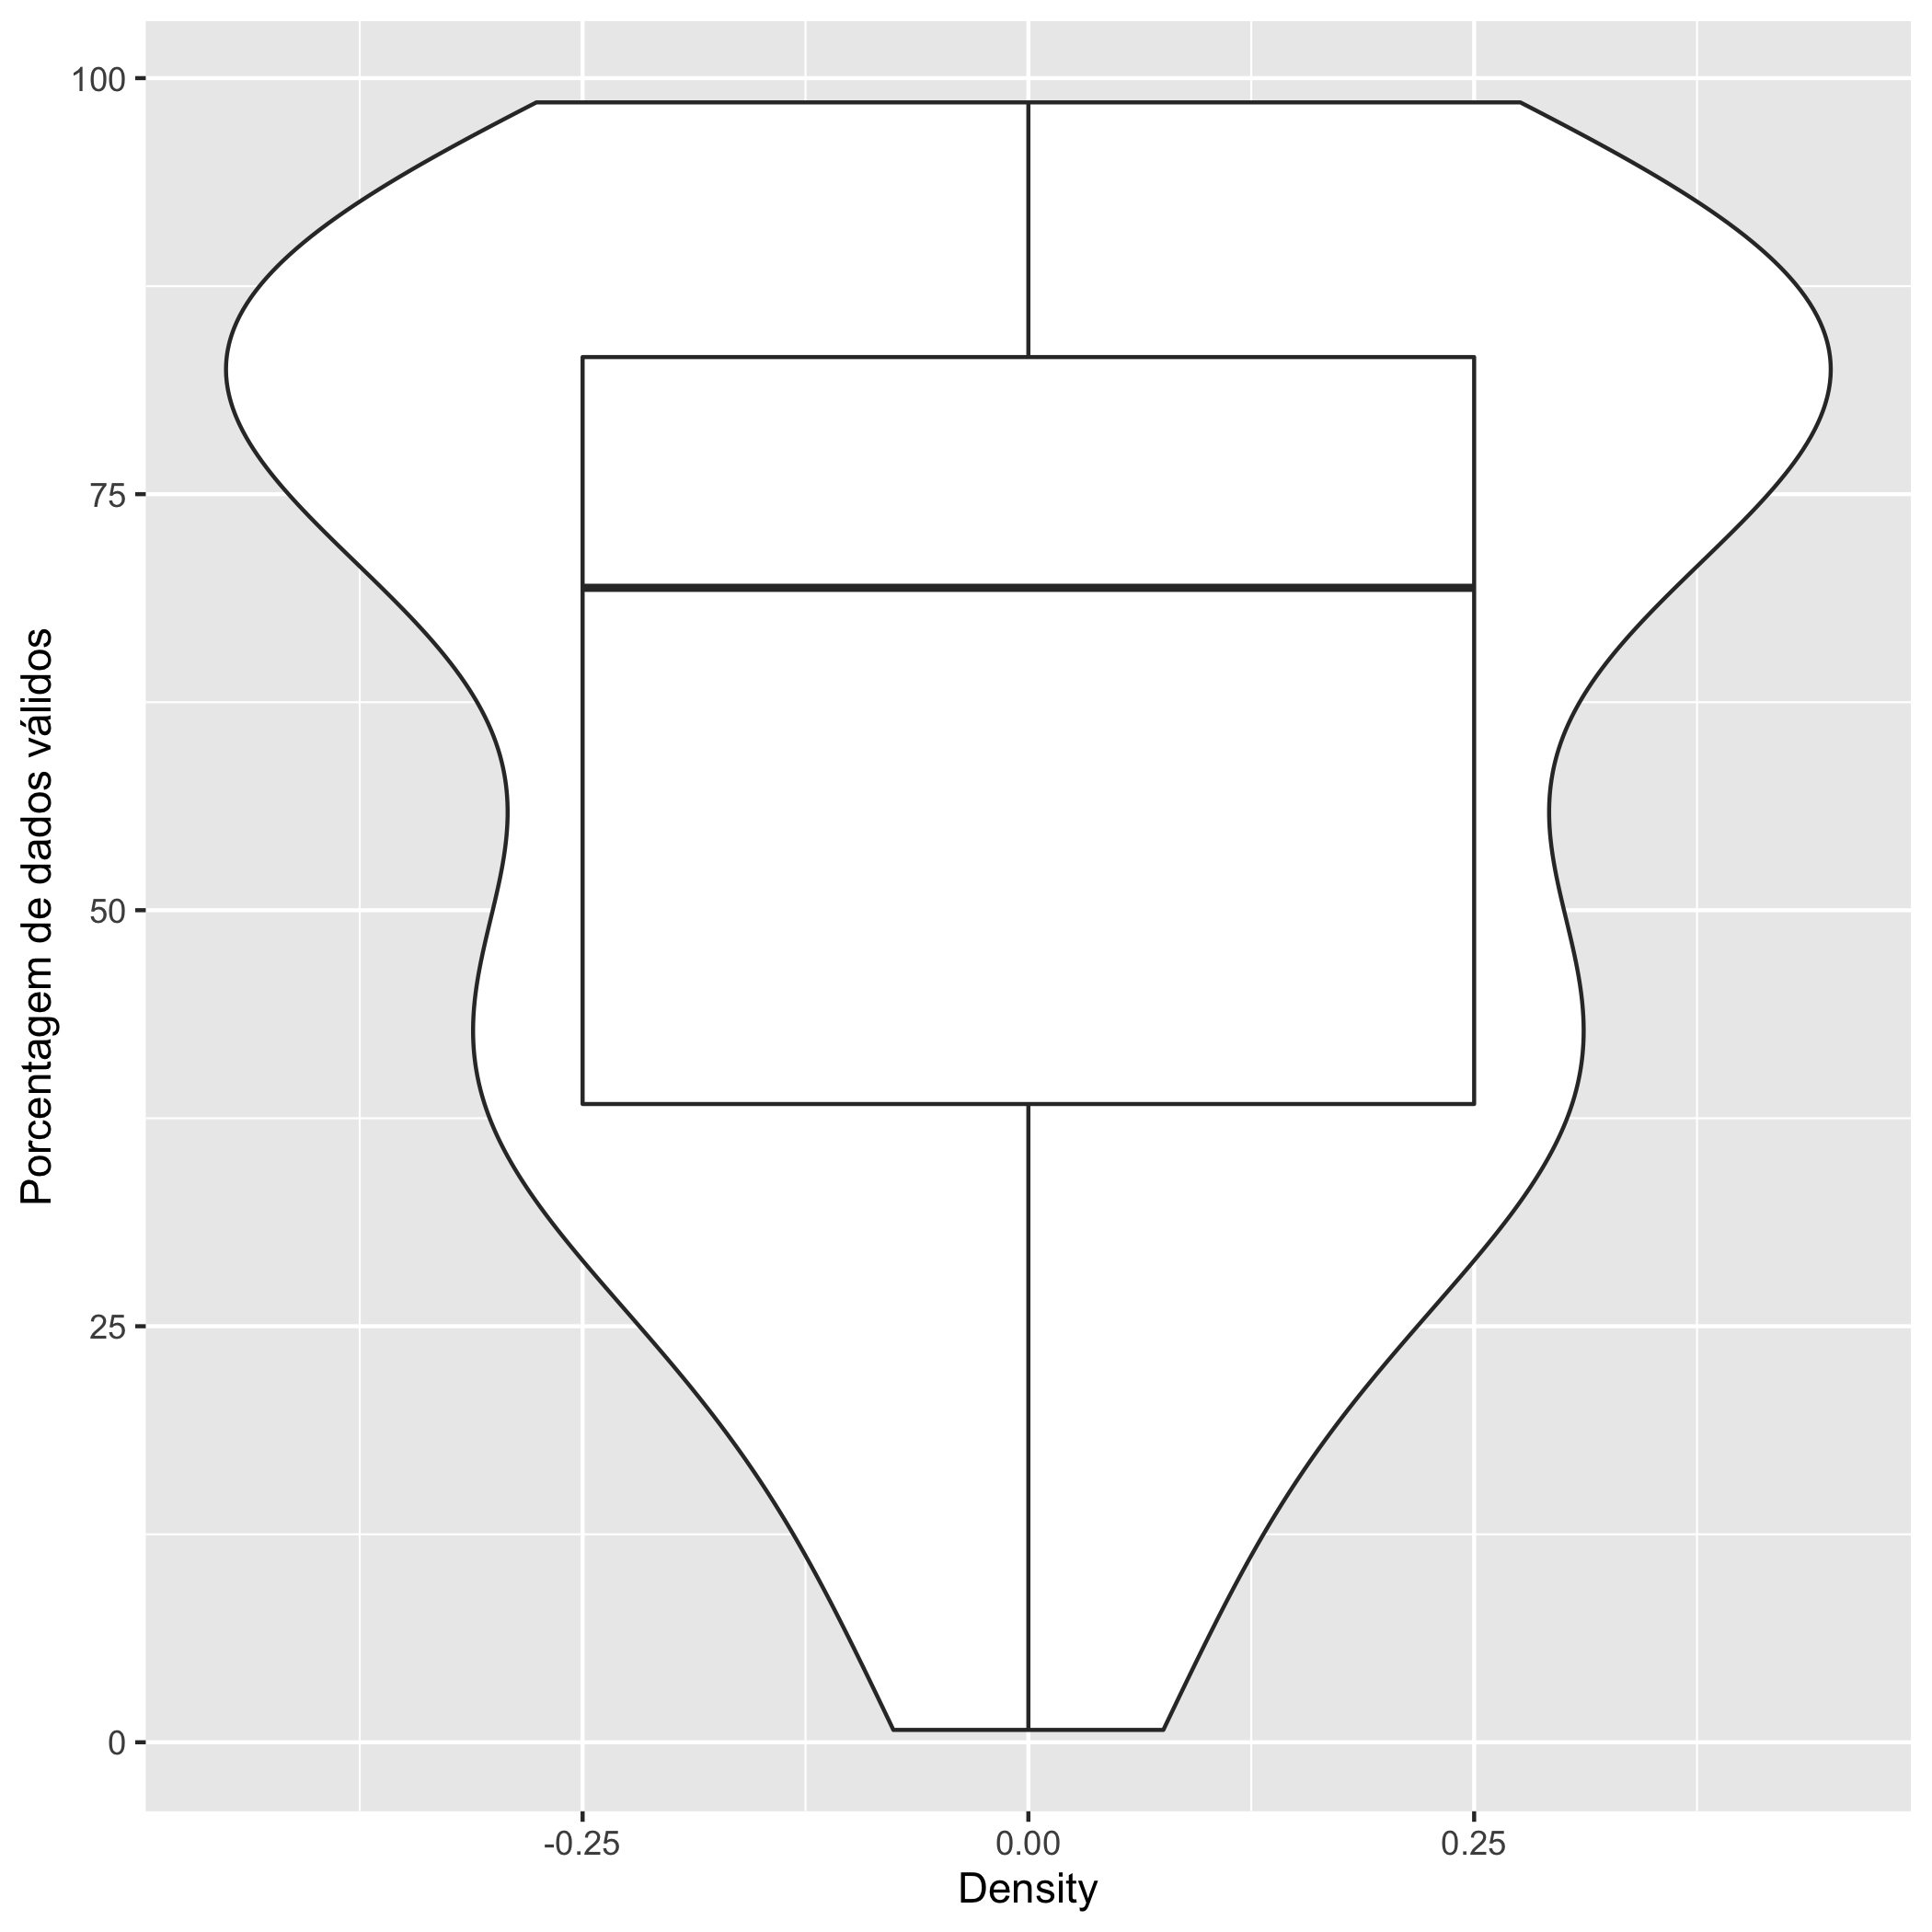
\includegraphics[scale=0.2]{"./qualityCheckFigure1.png"}}
\centering
\end{figure}

\begin{figure}[t]
\caption{Incluindo baseline e transições}
\noindent\makebox[\textwidth]{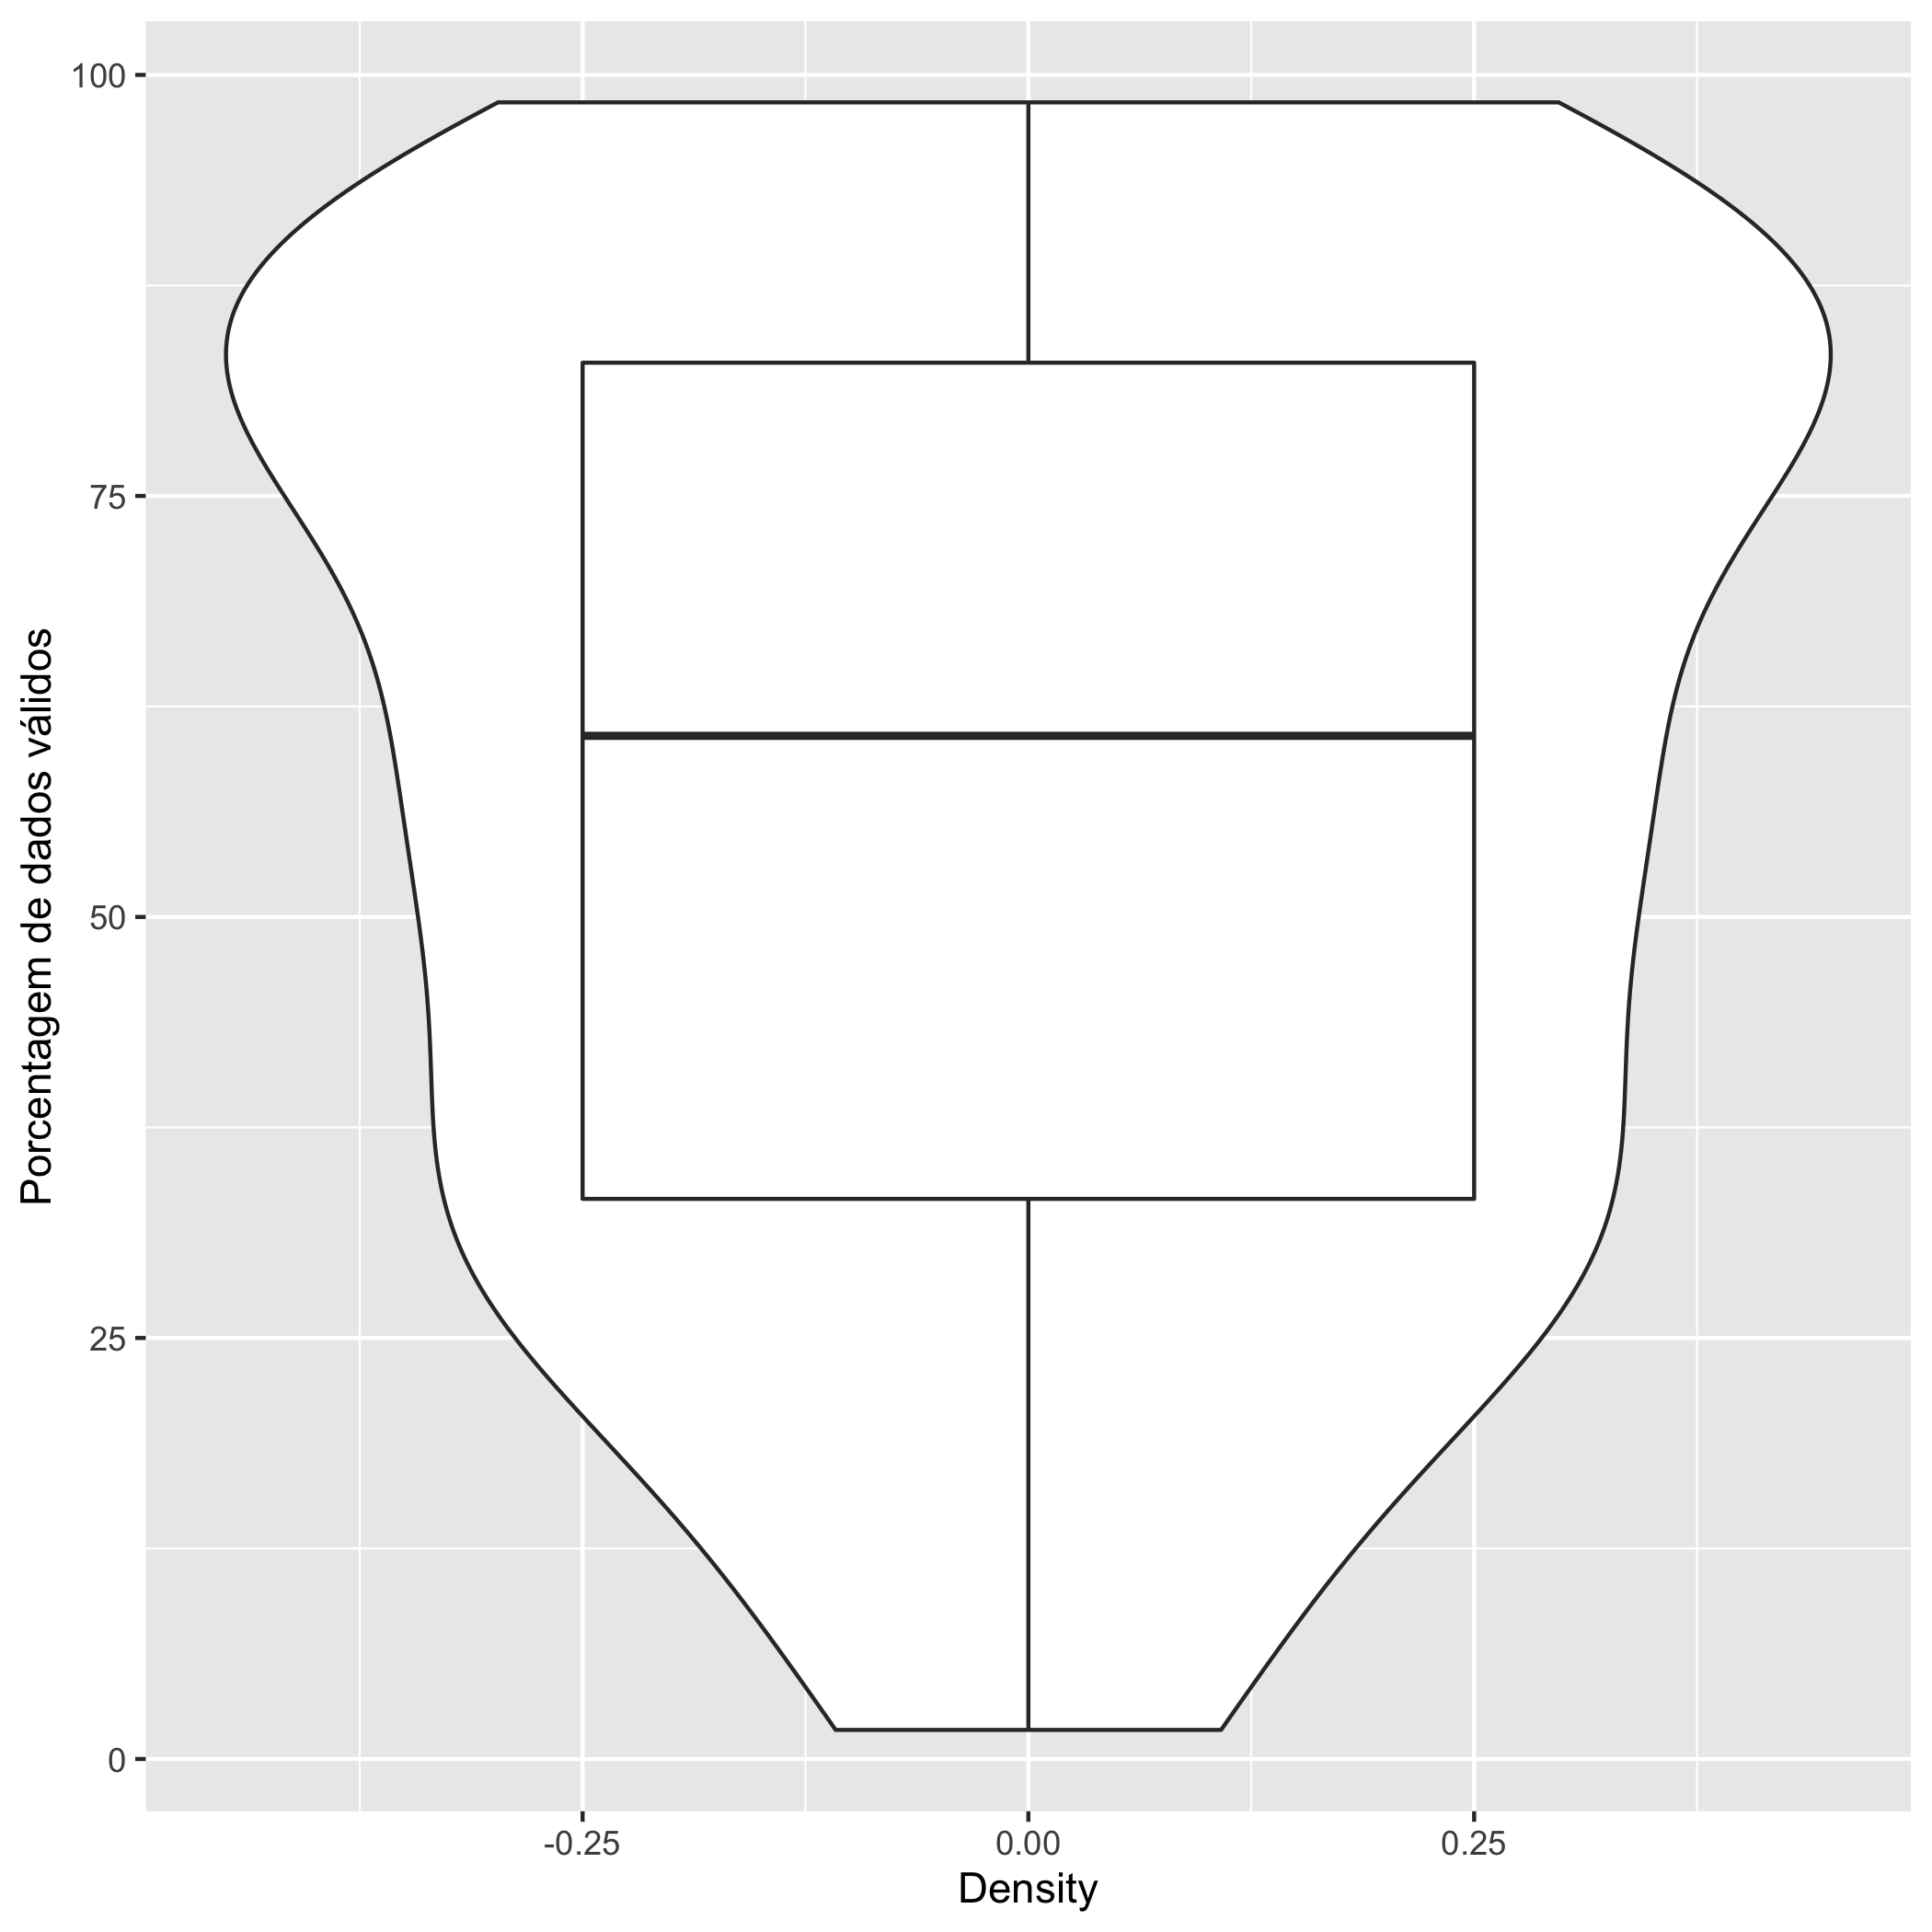
\includegraphics[scale=0.2]{"./qualityCheckFigure2.png"}}
\centering
\end{figure}

\begin{figure}[t]
\caption{Exemplo de fixações realizadas por um participante. Eixo x representa o tempo, eixo y o local da tela onde o participante olhou. R (Rosto), BD(Brinquedo Direita), BE(Brinquedo Esquerda). Porcentagem de fixações corretas = 37.43\%}
\noindent\makebox[\textwidth]{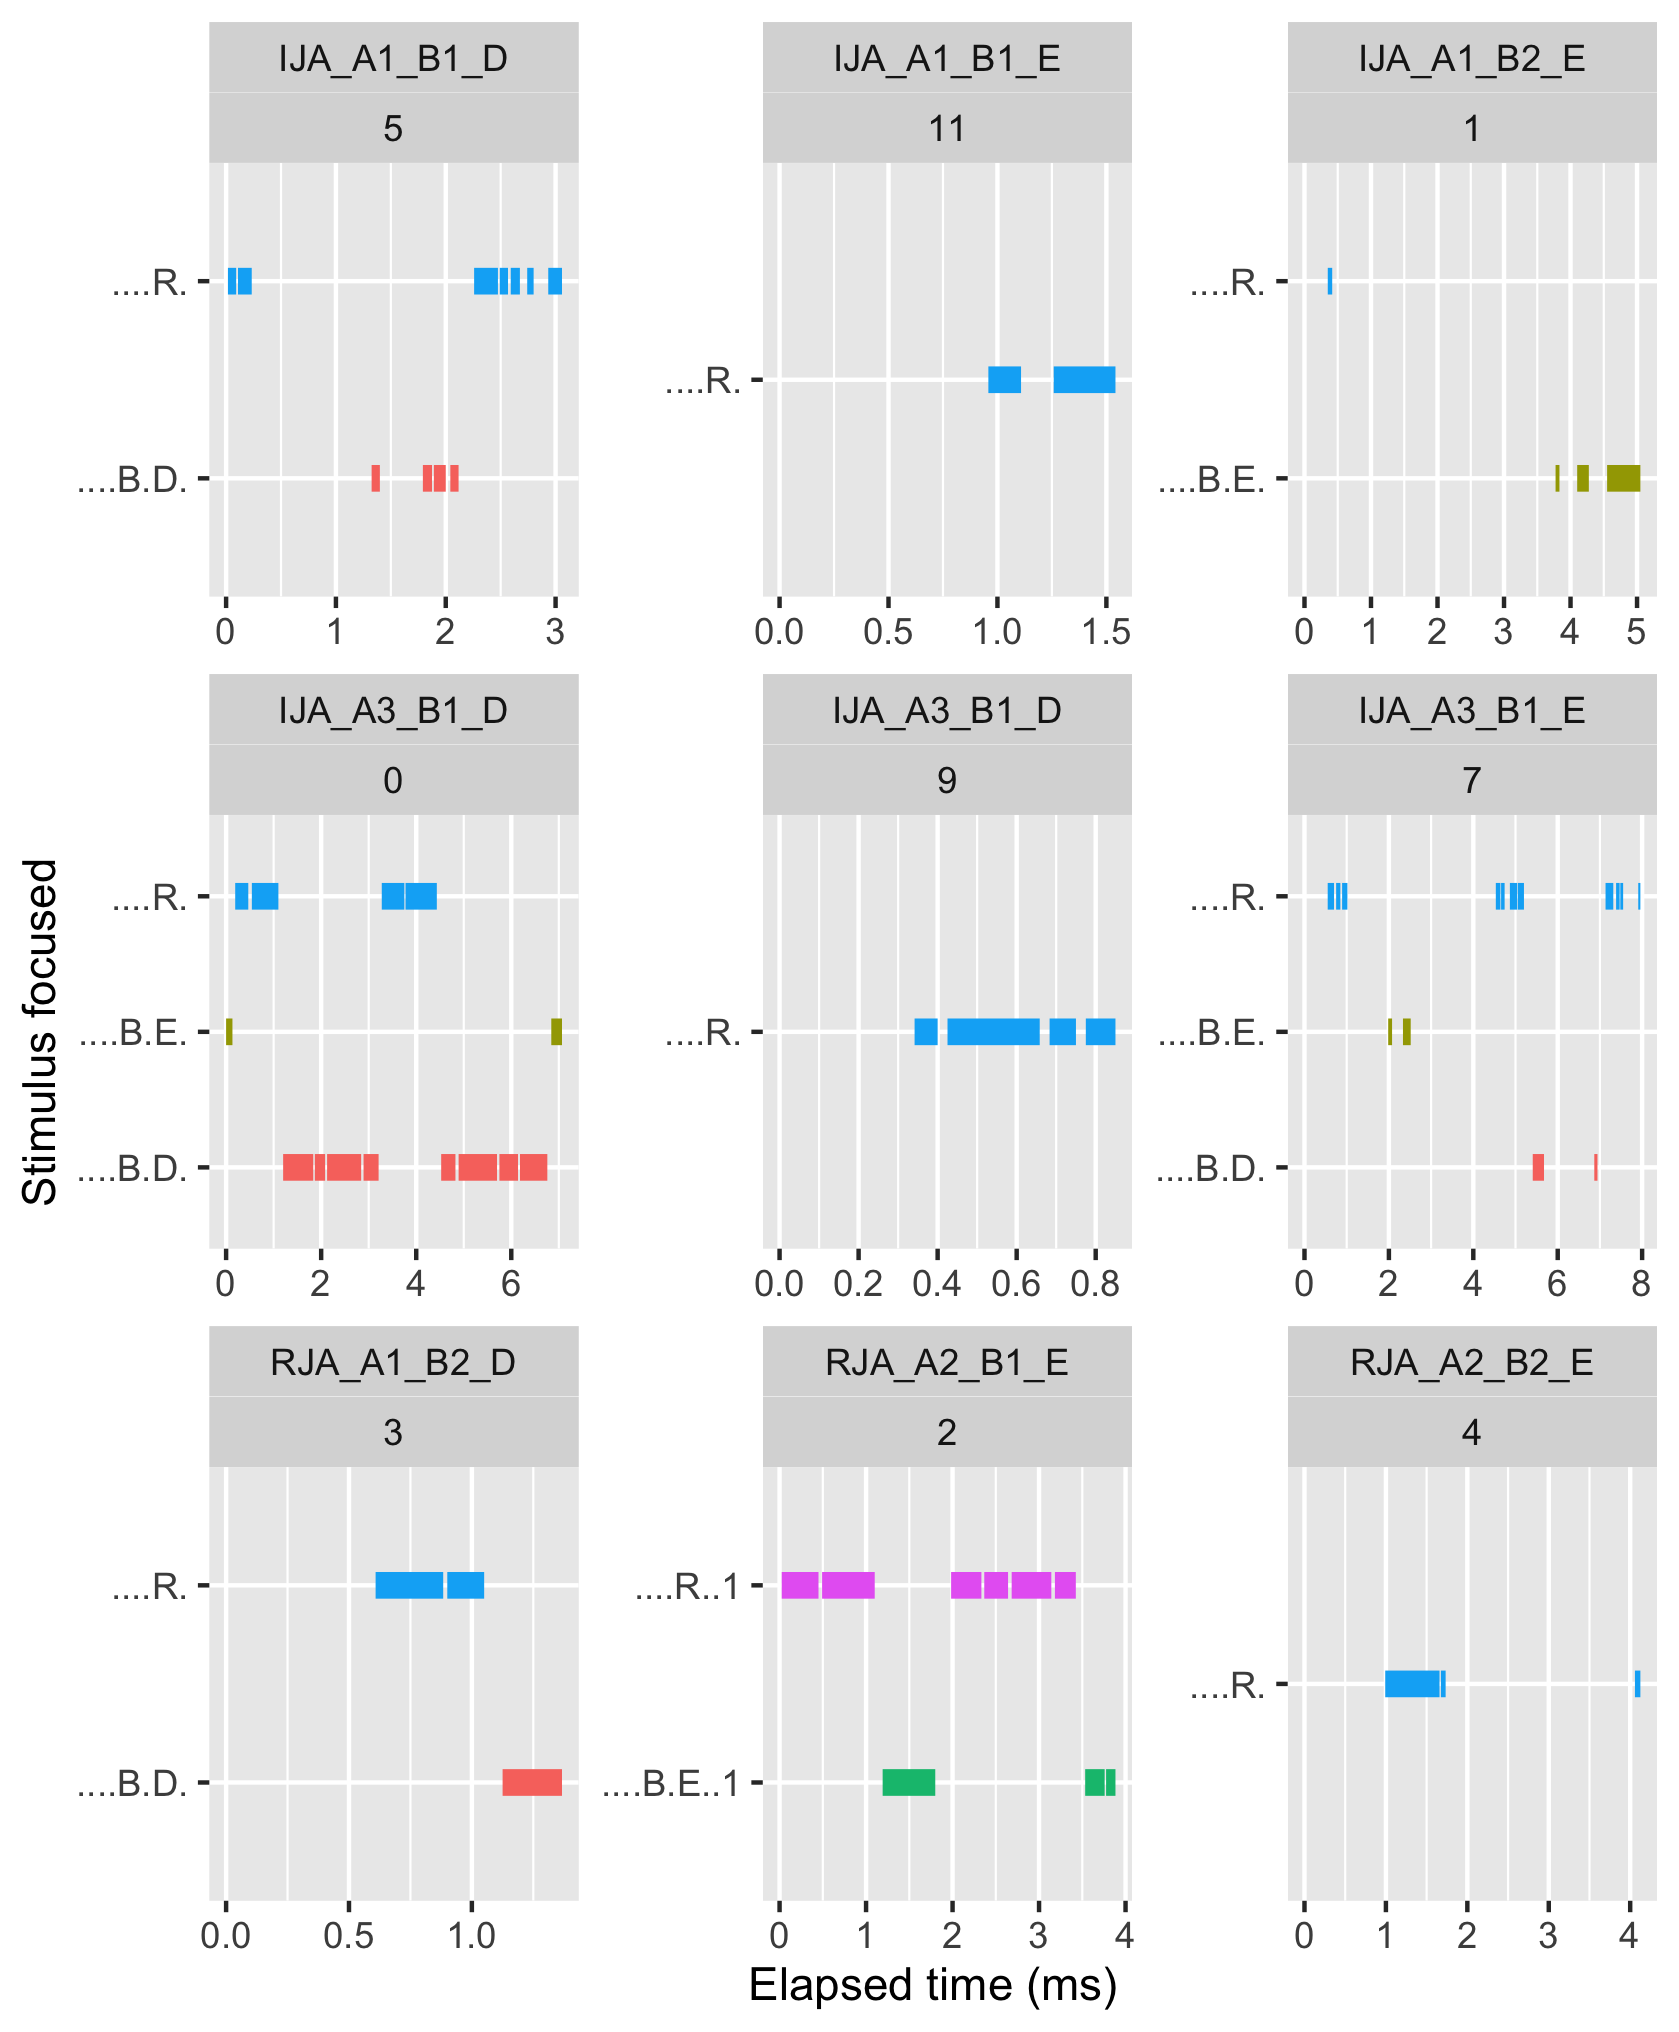
\includegraphics[scale=0.30]{"./exampleParticipant.png"}}
\centering
\end{figure}


\end{document}


